\documentclass[12pt,a4paper]{article} 
\usepackage{a4wide}
\usepackage[utf8]{inputenc}
\usepackage{amsmath}
\usepackage{amsfonts}
\usepackage{amssymb}
\usepackage{graphicx}
\usepackage{float}
\usepackage[ngerman]{babel} 
\usepackage{pdflscape}
\usepackage{caption, booktabs}
\parindent0pt


\title{Teilentwurf von  LISE E-Learning System}

\author{Matthias Englert, Fabian Schilha, Andreas Rottach}
\date{Wintersemester 2014/2015}

\begin{document}
\maketitle
\newpage
\tableofcontents
\newpage

\section{Datenbankentwurf}

\subsection{Datebankdiagramm}
\begin{figure}[H]
	\centering
	\paragraph{Aufbau der Relationalen Datenbank}	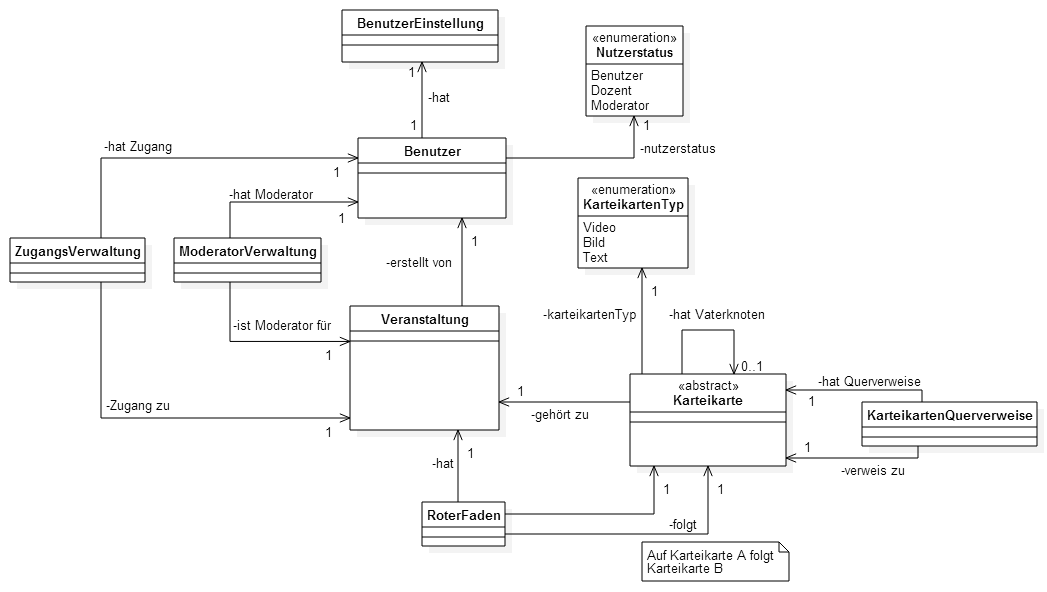
\includegraphics[width=\textwidth]{Bilder/Datenbank/Datenbankentwurf.png}
	\caption{Datenbankdiagramm}
	\label{Datenbankdiagramm}
\end{figure}

\subsection{Beschreibung der Tabellen}
\begin{tabular}{|lp{12cm}|}
	\hline
	TABELLE			&  Veranstaltung\\ 
	BESCHREIBUNG	&  Speichert alle Veranstaltungen an der Universität Ulm\\ 
	VERWALTET		&  Veranstaltungsinformationen und -einstellungen\\ 
	SCHLÜSSEL		&  ID : Integer\\ 
	\hline
	&  \\ 
	FELD		    &  Titel : String\\  
	&  \\
	FELD		    &  Beschreibung : String\\ 
	BESCHREIBUNG	&  Veranstaltungsbeschreibung\\
	&  \\
	FELD		    &  Studiengang : Enum\\ 
	BESCHREIBUNG	&  Veranstaltung ist bestimmten Studiengängen zugeordnet\\ 
	&  \\
	FELD		    &  Semester : String\\ 
	BESCHREIBUNG	&  Semsterinformationen werden im Format \glqq WS/SS JAHR\grqq gesichert \\
	&  \\
	FELD		    &  Zugangspasswort : String\\ 
	BESCHREIBUNG	&  speichert das verschlüsselte Passwort der Veranstaltung\\
	&  \\
	FELD		    &  DisskusionErlaubt : Boolean\\ 
	BESCHREIBUNG	&  True lässt Diskussionen zu, False deaktiviert diese Möglichkeit \\
	&  \\
	FELD		    &  BewertungenErlaubt : Boolean\\ 
	BESCHREIBUNG	&  True lässt Bewertungen zu, False deaktiviert diese Möglichkeit \\
	&  \\
	FELD		    &  GruppenErlaubt : Boolean\\ 
	BESCHREIBUNG	&  True lässt Gruppen zu, False deaktiviert diese Möglichkeit \\
	&  \\
	FELD		    &  GruppenErlaubt : Boolean\\ 
	BESCHREIBUNG	&  True lässt Gruppen zu, False deaktiviert diese Möglichkeit \\
	&  \\
	FELD		    &  ModeratorKarteikartenBearbeiten : Boolean\\ 
	BESCHREIBUNG	&  True Bearbeitungen von dem Moderator zu, False deaktiviert diese Möglichkeit. Dann kann er nur Diskussionen verwalten. \\
	&  \\
	FELD		    &  ModeratorKarteikartenBearbeiten : Boolean\\ 
	BESCHREIBUNG	&  True Bearbeitungen von dem Moderator zu, False deaktiviert diese Möglichkeit. \\
	&  \\
	FELD		    &  ErstellerID : Benutzer\\ 
	BESCHREIBUNG	&  Fremdschlüssel, Verweis auf den Dozenten, der diese Veranstaltung erstellt hat. \\
	\hline
\end{tabular}\\\\

\begin{tabular}{|lp{12cm}|}
	\hline
	TABELLE			&  Benutzer\\ 
	BESCHREIBUNG	&  Speichert alle Informationen, die zu einem Benutzer gehören.\\ 
	VERWALTET		& Benutzerdaten\\ 
	SCHLÜSSEL		&  ID : Integer\\ 
	\hline
	&  \\ 
	FELD		    &  Vorname : String\\  
	&  \\ 
	FELD		    &  Nachname : String\\  
	&  \\ 
	FELD		    &  Martrikelnummer : Integer\\  
	&  \\
	FELD		    &  eMail : String\\ 
	BESCHREIBUNG	&  Veranstaltungsbeschreibung\\
	&  \\
	FELD		    &  Studiengang : Enum\\ 
	BESCHREIBUNG	&  Benutzer ist bestimmtem Studiengang zugeordnet. Dozenten sind hier keinem Studiengang zugeordnet.\\ 
	&  \\
	FELD		    &  Kennwport : String\\ 
	BESCHREIBUNG	&  Speichert das verschlüsselte Passwort des Nutzers \\
	&  \\
	FELD		    &  Nutzerstatus : Enum\\ 
	BESCHREIBUNG	&  Speichert ob Benutzer ein Student oder Dozent ist.\\
	&  \\
	FELD		    &  GruppeneinladungenErlauben : Bool\\ 
	BESCHREIBUNG	&  Speichert ob Benutzer zu Gruppen eingeladen werden kann.\\
	&  \\
	FELD		    &  NotifyDiskussionen : Enum\\ 
	BESCHREIBUNG	&  Speichert wie ein Benutzer über Diskussionen informiert wird.\\
	\hline
\end{tabular}\\\\

\begin{tabular}{|lp{12cm}|}
	\hline
	TABELLE			&  Karteikarte\\ 
	BESCHREIBUNG	&  Speichert alle Informationen die zu einer Karteikarte gehören.\\ 
	VERWALTET		&  Karteikartendaten\\ 
	SCHLÜSSEL		&  ID : Integer\\ 
	\hline
	&  \\ 
	FELD		    &  Titel : String\\  
	&  \\
	FELD		    &  KarteikartenTyp : Enum\\ 
	BESCHREIBUNG	&  Speichert, ob es sich um Text-, Bild- oder Videomaterial handelt.\\
	&  \\
	FELD		    &  Aenderungsdatum : Date\\ 
	BESCHREIBUNG	&  Datum an dem die Karteikarte zuletzt editiert wurde.\\ 
	&  \\
	FELD		    &  Inhalt : String\\ 
	BESCHREIBUNG	&  Enthält Text oder Dateipfad zu der Bild- bzw. Video-Datei.\\
	\hline
\end{tabular}\\\\

\begin{tabular}{|lp{12cm}|}
	\hline
	TABELLE			&  ZugangsVerwaltung\\ 
	BESCHREIBUNG	&  Verwaltet, welcher Benutzer zu welcher Veranstaltung Zugang hat.\\ 
	VERWALTET		&  Zugang zu Veranstaltungen\\ 
	SCHLÜSSEL		&  ID : Integer\\ 
	\hline
	&  \\
	FELD		    &  NutzerID : Benutzer\\ 
	BESCHREIBUNG	&  Fremdschlüssel, Referenz auf Benutzer.\\
	&  \\
	FELD		    &  VeranstaltungID : Veranstaltung\\ 
	BESCHREIBUNG	&  Fremdschlüssel, Referenz auf Veranstaltung.\\
	\hline
\end{tabular}\\\\

\begin{tabular}{|lp{12cm}|}
	\hline
	TABELLE			&  ModeratorVerwaltung\\ 
	BESCHREIBUNG	&  Verwaltet, welcher Benutzer als Moderator für eine Veranstaltung tätig ist.\\ 
	VERWALTET		&  Zuordnung zwischen Moderator und Veranstaltung\\ 
	SCHLÜSSEL		&  ID : Integer\\ 
	\hline
	&  \\
	FELD		    &  ModeratorID : Benutzer\\ 
	BESCHREIBUNG	&  Fremdschlüssel, Referenz auf Benutzer.\\
	&  \\
	FELD		    &  VeranstaltungID : Veranstaltung\\ 
	BESCHREIBUNG	&  Fremdschlüssel, Referenz auf Veranstaltung.\\
	\hline
\end{tabular}\\\\

\begin{tabular}{|lp{12cm}|}
	\hline
	TABELLE			&  KarteikartenQuerverweise\\ 
	BESCHREIBUNG	&  Verwaltet die Querverweise zwischen Karteikarten.\\ 
	VERWALTET		&  Zuordnung zwischen Karteikarte und Karteikarte(Querverweis).\\ 
	SCHLÜSSEL		&  ID : Integer\\ 
	\hline
	&  \\
	FELD		    &  KarteikarteID : Karteikarte\\ 
	BESCHREIBUNG	&  Fremdschlüssel, Referenz auf Karteikarte.\\
	&  \\
	FELD		    &  QuerverweisID : Karteikarte\\ 
	BESCHREIBUNG	&  Fremdschlüssel, Referenz auf Karteikarte.\\
	\hline
\end{tabular}\\\\

\begin{tabular}{|lp{12cm}|}
	\hline
	TABELLE			&  KarteikarteAttribteZuordnung\\ 
	BESCHREIBUNG	&  Verwaltet die Zuordnung zwischen Attributen und einer Karteikarte.\\ 
	VERWALTET		&  Zuordnung zwischen Karteikarte und Attribute.\\ 
	SCHLÜSSEL		&  ID : Integer\\ 
	\hline
	&  \\
	FELD		    &  KarteikarteID : Karteikarte\\ 
	BESCHREIBUNG	&  Fremdschlüssel, Referenz auf Karteikarte.\\
	&  \\
	FELD		    &  Attribut : Enum\\ 
	BESCHREIBUNG	&  Dieser Enum speichert das gesetzte Attribut.\\
	\hline
\end{tabular}\\\\

\begin{tabular}{|lp{12cm}|}
	\hline
	TABELLE			&  RoterFaden\\ 
	BESCHREIBUNG	&  Speichert die Reihenfolge der Karteikarten im Roten Faden einer Veranstaltung.\\ 
	VERWALTET		&  Karteikarten.\\ 
	SCHLÜSSEL		&  ID : Integer\\ 
	\hline
	&  \\
	FELD		    &  KarteikarteID : Karteikarte\\ 
	BESCHREIBUNG	&  Fremdschlüssel, Referenz auf Karteikarte.\\
	&  \\
	FELD		    &  NachfolgerID : Karteikarte\\ 
	BESCHREIBUNG	&  Fremdschlüssel, Referenz auf Karteikarte die im Roten Faden folgt.\\
	&  \\
	FELD		    &  VeranstaltungID : Veranstaltung\\ 
	BESCHREIBUNG	&  Fremdschlüssel, Referenz auf zugehörige Veranstaltung.\\
	\hline
\end{tabular}\\\\


\section{System-Architektur}

\subsection{Kommunikationsdiagramm}

\subsection{Klassendiagramm}

\begin{figure}[H]
	\centering
	\paragraph{Klassendiagramm}
	%	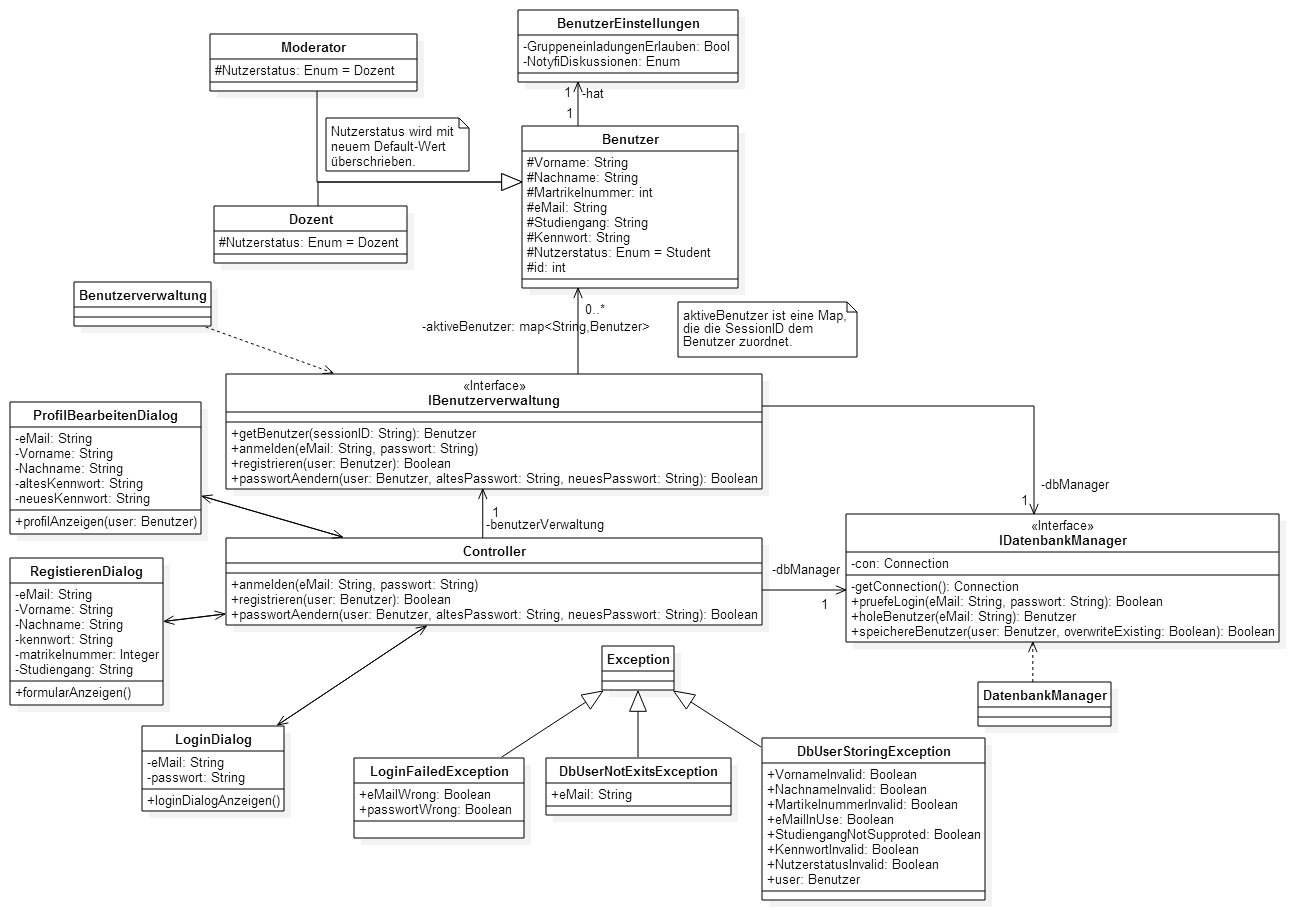
\includegraphics[width=\textwidth]{Bilder/Klassendiagramm/Klassendiagramm.png}
	\caption{Klassendiagramm}
	\label{Klassendiagramm des Teilsystems}
\end{figure}

\subsection{Methodenbeschreibung}


\begin{tabular}{|lp{12cm}|}
			\hline
			Operation &  \textbf{registrieren(neuerNutzer: Benutzer): Boolean }\\ 
			Beschreibung & Ein Benutzer registriert sich neu im System und gibt alle verlangten Daten an. Die Operation prüft ob die Daten korrekt sind und legt den neuen Benutzer gegebenenfalls an.\\ 
			Erzeugt &  Benutzer\\ 
			Pre &  Nutzer ist noch nicht registriert. \\ 
			Post & Nutzer ist im System angelegt.  \\ 
			\hline 
\end{tabular} \\\\



\end{document}
